\section{Workload Generation}
\label{se:workload}

As explained in the research methodology (in \cref{subse:timeseries_key_attributes}), we selected six primary attributes from the timeseries metadata while implementing the system architecture. Before storing the data in \acrshort{wdias}, we need to register timeseries metadata for the timeseries, and are required to provide values for the six attributes. During the test for location attribute, we selected set of locations all over the world as a generic case to include all the locations without binding to a specific area.

We used 250 locations from Google’s countries public data set \cite{GoogleGoogleCounties}, and considered static throughout the testing. For each location, we created four timeseries metadata by using four different values for the moduleId key attribute. Thus, combining all together first, we created 1000 timeseries metadata during the performance test and then stored the timeseries data against timeseries unique identifiers. We have written automated scripts to generate these data for the performance testing, and scripts are generic enough to create more timeseries metadata by changing the configurations.

For storing grid data, we used static 100 grid locations. Since grid locations have different metadata structures, we had to generate metadata for them separately. However, the locationID of the grid timeseries metadata is similar to scalar timeseries metadata that have the same effect when defining timeseries metadata.

We used the Apache JMeter 5.0 version \cite{ApacheSoftwareFoundationApacheJMeter} for performing the load test since it is a widely using open source tool which supports distributed load testing. As mentioned in the JMeter best practices, "If your test needs large amounts of data - particularly if it needs to be \emph{randomized}, create the test data in a file that can be read with CSV data set. This avoids wasting resources at run-time". While running the load test, JMeter iterates over the timeseries metadata CSV file and assigns a new thread to work on the test scenario with given timeseries metadata. Instead of providing the randomness at run time, we stored the timeseries metadata in random order that satisfies the percentage of 70\% scalar, 20\% vector, and 10\% grid, as mentioned in \cref{se:test_plan}.
Before running the test cases, we generated the timeseries metadata in random order and wrote them into a CSV file during the setup phase. The metadata CSV file arranges in a way that, within every ten lines, seven lines are scalar timeseries, two lines are vector timeseries, and 1 line is a grid timeseries.

\acrshort{wdias} is capable of storing any numeric value up to 3 decimal points as per the default configuration. Even the parameter type is either precipitation, temperature does not make any difference, because in storage perspective, we are storing numeric value. Thus, during the performance testing, we only use real precipitation data from \acrshort{curw}. So, we used data from five weather stations for a month while preparing the test data for scalar timeseries. We used a script to clean up and prepare the precipitation data, and it is available as setup precipitation in \acrshort{wdias} codebase.

\begin{minipage}{\linewidth}
\begin{lstlisting}[language=sh, caption=Preparation of precipitation data.]
Set ROOT_DIR=~/wdias/wdias-performance-test
-h | --help: Usage
  setup_precipitation.sh  <COMMAND>
    - COMMAND: help | extract | prepare | cleanup | populate
  e.g.
  setup_precipitation.sh prepare
    Segregate single file data into multiple files based on date. And Separate into main directories of 15min, 30min, 60min and create tar files
  setup_precipitation.sh extract
    Extract the tar files into 15min, 30min and 60min
  setup_precipitation.sh cleanup
    Clean up extracted directories
\end{lstlisting}
\end{minipage}

While preparing the data, we created three sets of timeseries based on the time interval, such as hourly (60-minute), 30-minute, and 15-minute data, with modifying the replicated data. The above method reduced the overhead of filtering data during performance testing. We also set up the JMeter as a containerized application, which allows us to run inside the k8s cluster. As an optimization for the JMeter container creation, we avoid adding extensive test timeseries data, which causes the container size to be large and making the build process slower. Rather than doing that, we used extract scripts while running the container and extract the data into the container. For each test plan, we used a date counter and increment the date after one full cycle of timeseries metadata CSV file is processed. When the date counter increases, it reads the real data for that day. After the date counter advances to the next month, we repeat reading data from the beginning of the month. To provide more randomness, we switch over five locations during the date increment. The JMeter reads the data via the JSR223 scripts, and we have written those scripts in a generalized style such that it is possible to tweak and use if there are more location data available.

Similar to the scalar test data prepared, we prepared the test grid data using the real water-level output of the FLO2D 150 meter hydrology model that is used in the \acrshort{curw}. The FLO2D timeseries are produced as ASCII Grid files, and each data point represents a grid file that consists of 120 rows and 139 columns. To represent missing cell values of the ASCII grid file, we used the \texttt{-9} instead of \texttt{-999} as an optimization. Even with that, each file size is around 50,337 Bytes (50 Kilobytes).

\begin{minipage}{\linewidth}
\begin{lstlisting}[language=sh, caption= Preparation of water-level data.]
Set ROOT_DIR=~/wdias/wdias-performance-test
-h | --help: Usage
  setup_water-level.sh  <COMMAND>
    - COMMAND: help | extract | prepare | cleanup | populate
  e.g.
  setup_water-level.sh prepare
    Segregate single file data into multiple grid file directories based on date. And Separate into main directories of 15min, 30min, 60min and create tar files
  setup_water-level.sh extract
    Extract the tar files into 15min, 30min and 60min
  setup_water-level.sh cleanup
    Clean up extracted directories
\end{lstlisting}
\end{minipage}

We also used the real water level data for one month period and developed a script to do the data preparation, cleanup, and extract. Similar to the scalar test scenario, the JMeter repeats reading from the beginning of test data when the date counter increments to the next month.


%%%%%%%%%%%%%%%%%%%%%%%%%%%%%%%%%%%%%%%%%%%%%%%%%%%%%%%%%%%%%%%%%%%%%%%%%%%%%%%%
\subsection{Experimental Setup}
\label{subse:experimental_setup}

To create a higher workload, we used JMeter's distributed testing capabilities. JMeter uses the master-slave approach for distributed testing and allows us to handle all the test cases via a single master instance. However, it has the limitation of \emph{the same test plan runs by all the servers} rather than distributing the work among slave instances. In other words, JMeter does not distribute the load between servers, and each slave service runs the full test plan. So, if we set 1,000 threads per test plan and run the test using six JMeter servers, the distributed test setup ends up injecting 6,000 threads. During JMeter distributed mode, the master server triggers the same copy of the test plan on configured slave nodes in parallel. After successfully running the test plans, the master server gathers results from slave servers.

\begin{figure}[htp]
    \centering
    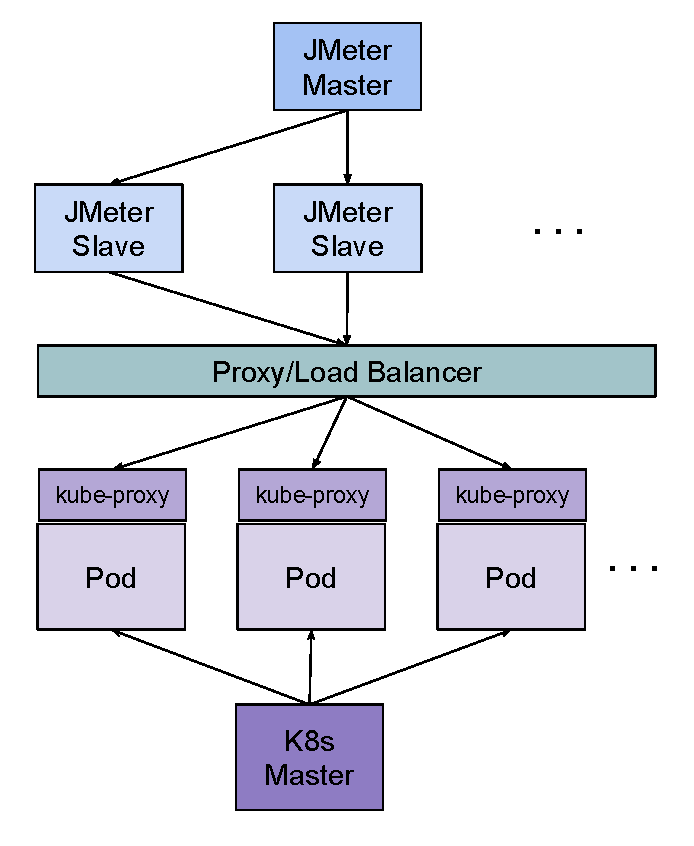
\includegraphics[width=0.6\textwidth]{results/work_load/experimental_setup_v3.pdf}
    \caption{Experimental setup with JMeter}
    \label{fi:experimental_setup}
\end{figure}

While implementing JMeter test plans, it uses threads to simulate the users. The root component of a test plan is the thread group. There are different kinds of thread groups available such as thread group (basic thread group), arrivals thread group, free form arrivals thread group, stepping thread group, concurrency thread group, and ultimate thread group.


%%%%%%%%%%%%%%%%%%%%%%%%%%%%%%%%%%%%%%%%%%%%%%%%%%%%%%%%%%%%%%%%%%%%%%%%%%%%%%%%
\subsubsection{Closed vs. Open Workload Models}
\label{subse:closed_vs_open_workload}

\begin{itemize}
    \item \emph{closed system model} \cite{Haggett1998AnWales} -- A new request is only triggered by the completion of a previous request, following by a think time. The system has negative feedback that makes it impossible to bury-out the service, so users wait for the responses before making new requests.
    \item \emph{open system model} -- New requests arrival independently of completions, e.g., according to a stochastic process or fixed trace. The system has no negative feedback.
\end{itemize}

While implementing the test cases for \acrshort{wdias}, we used the concurrency thread group with the throughput shaping timer extension of JMeter because it supports the open workload approach. Using other thread groups, we are required to find the exact number of threads and timer delays that produce the desired number of \acrshort{rps} to the server, which is known as the \emph{closed workload}. By using the \emph{throughput shaping timer}, we only need to configure the \acrshort{rps} throughout the test plan. Then the throughput shaping timer provides a feedback loop to the concurrency thread group via schedule feedback function to dynamically maintain thread count required to achieve target \acrshort{rps} \cite{KarunarathneGihanWdias/wdias-performance-test:JMeter.}.

\begin{figure}[htp]
    \centering
    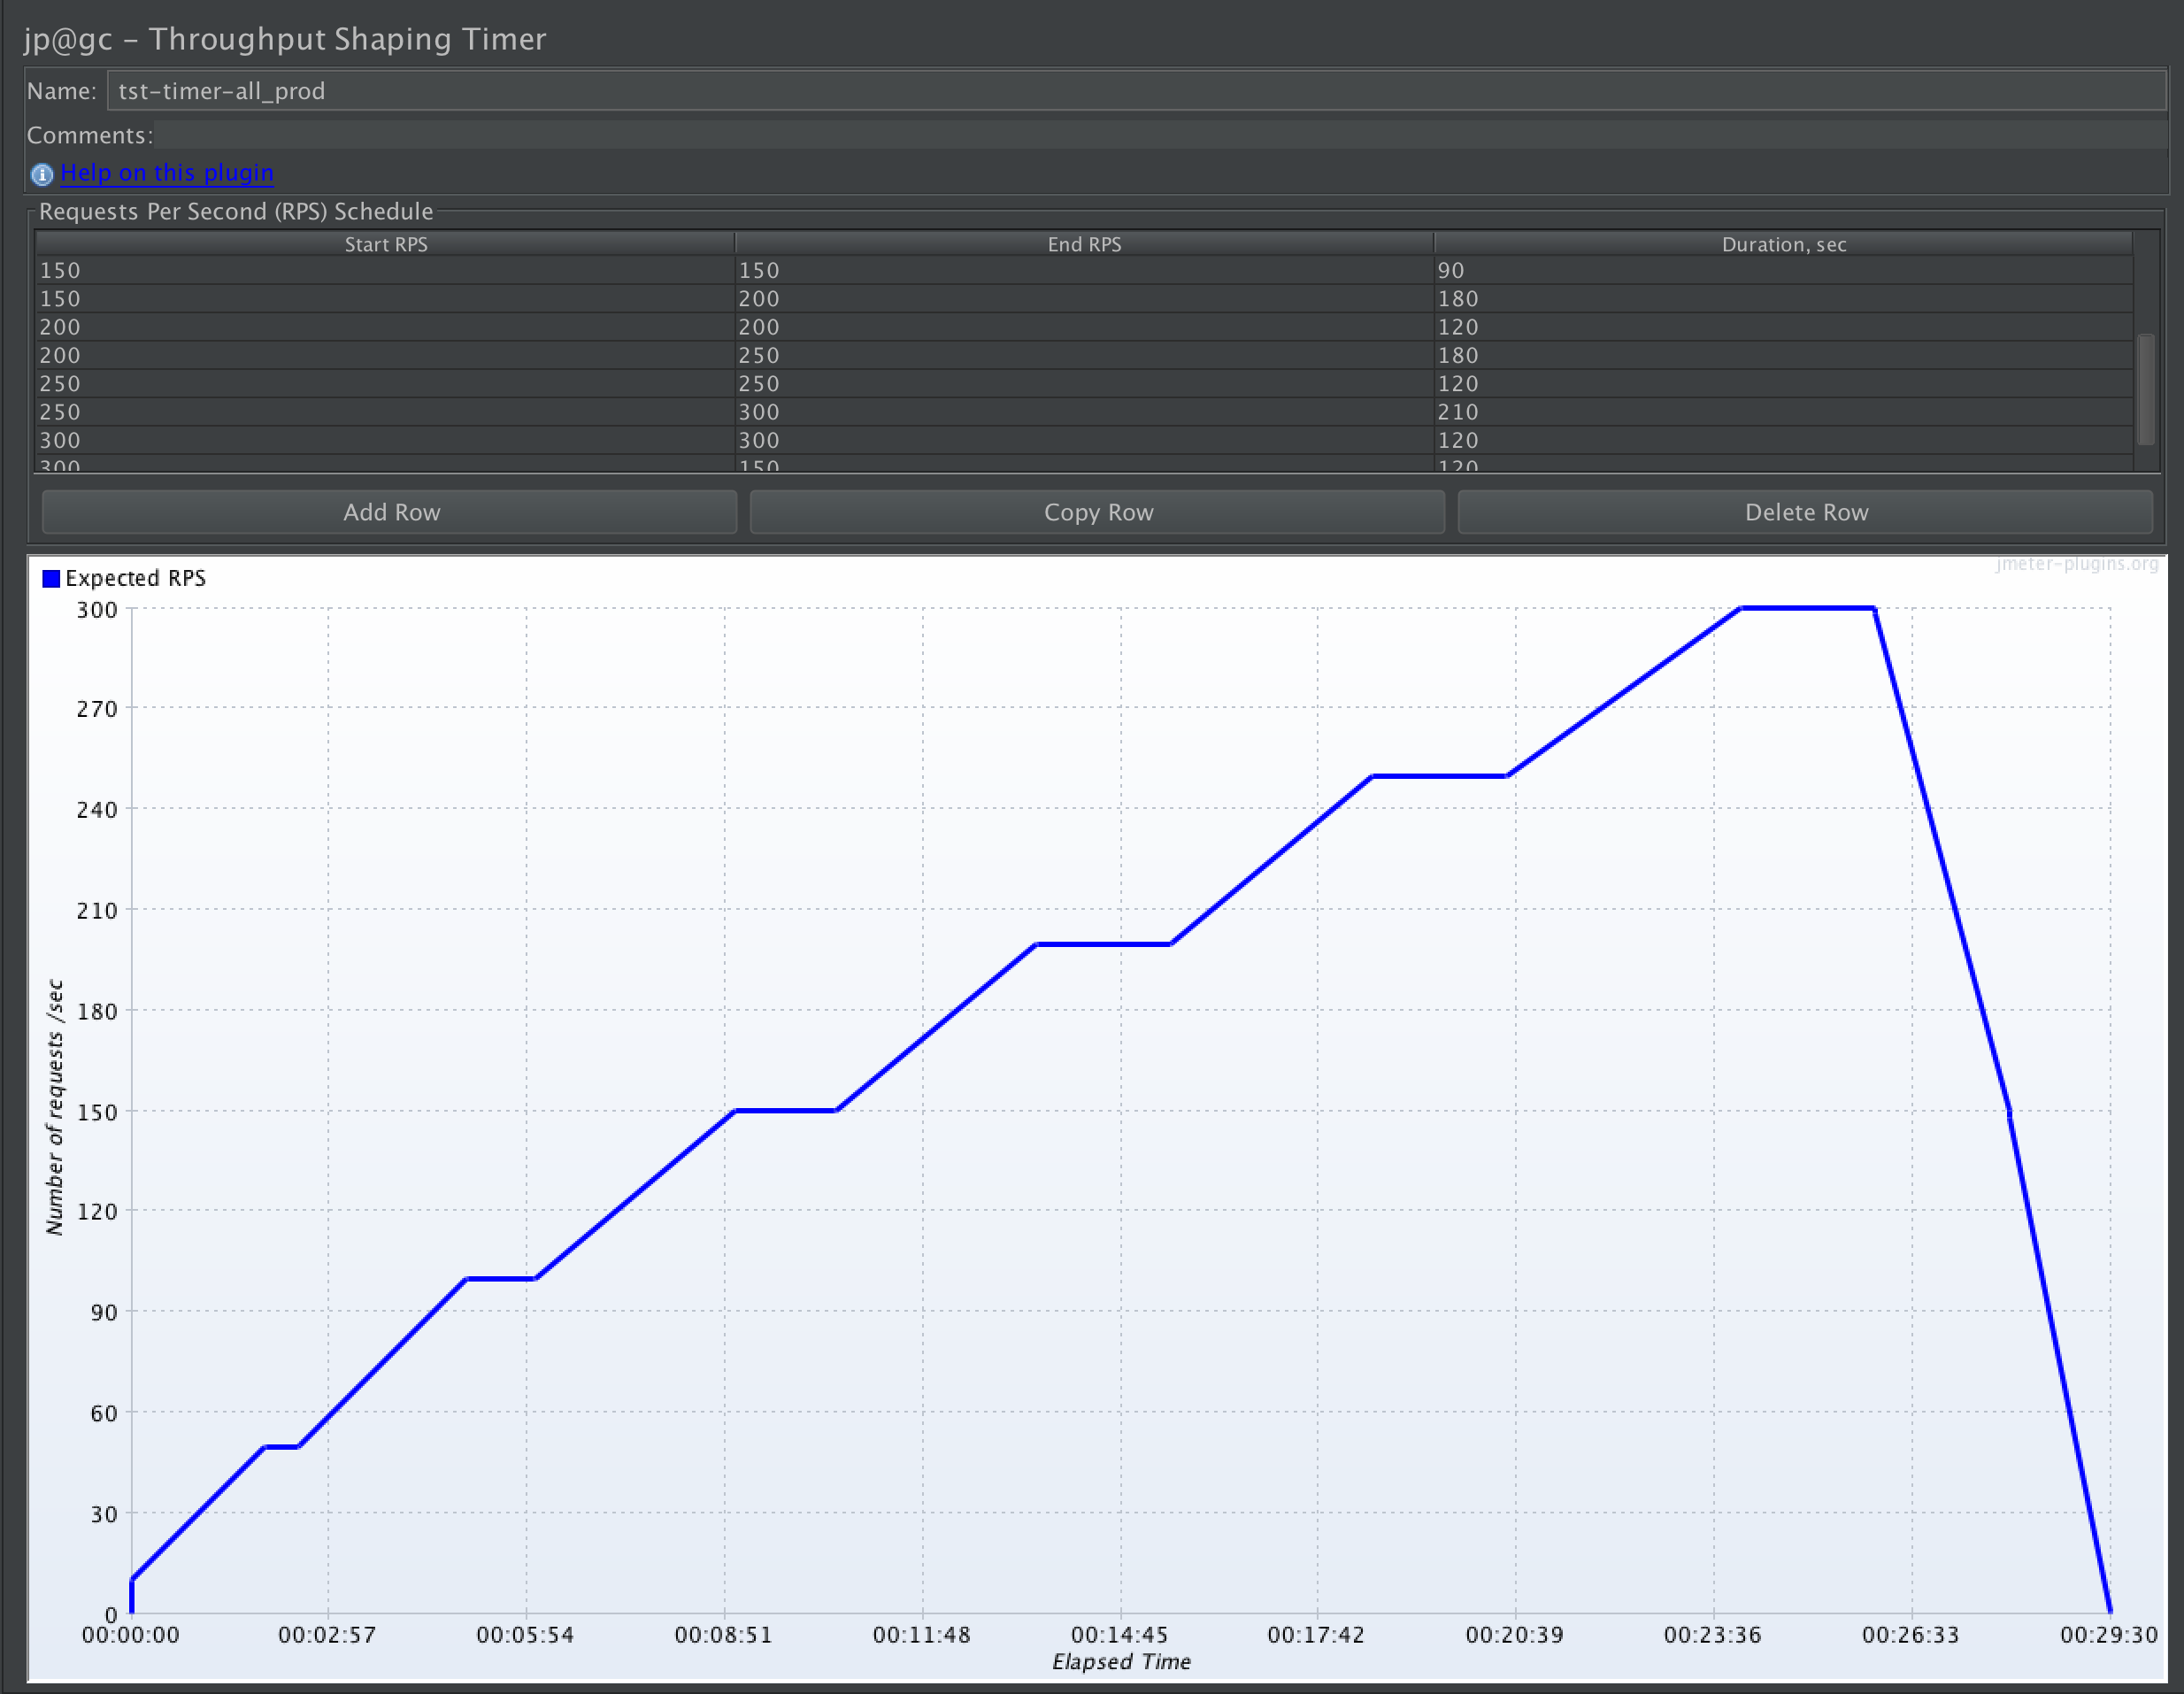
\includegraphics[width=0.8\textwidth]{results/work_load/test_prod_throughtput_shaping_timer.png}
    \caption{\acrshort{wdias} load testing throughput shaping timer \acrshort{rps} configurations.}
    \label{fi:test_prod_throughtput_shaping_timer}
\end{figure}

\cref{fi:test_prod_throughtput_shaping_timer} shows the throughput shaping timer configurations that we used for the load testing, and it is similar to the load test plan described in \cref{se:test_plan}. The maximum peak load that can be had during the load test is 300 \acrshort{rps} (equivalent to 18,000 requests per minute). The following the test plans that we used during the performance testing:

\begin{itemize}
    \item User-defined variables
    \item Setup thread group
    \item Create timeseries thread group
    \item Create extensions thread group
    \item Load test timeseries concurrency thread group
    \item Load test timeseries concurrency thread group
    \item Test flow thread group
\end{itemize}

The first step of the test plan consists of setting up the timeseries metadata. At the same time, we create the timeseries metadata in the \acrshort{wdias} system. Even with the real use case, users only have to register timeseries metadata once and reuse the generated timeseries identifier to insert the data. The following list of test steps shows the test plan for setting up the timeseries metadata.

\begin{itemize}
    \item HTTP request defaults
    \item HTTP header manager
    \item Timeseries metadata CSV
    \item Create timeseries
    \item Get timeseries
    \item Query timeseries
\end{itemize}

By creating the timeseries metadata before, we can reduce the overhead during the performance testing with only focus on essential data storing, and cause more accurate \acrshort{rps} at the run time. Otherwise, JMeter needs to allocate another set of threads for registering timeseries metadata. Further, when we consider real use cases, most of the time, the users want to search for timeseries metadata and retrieve relevant metadata, rather than registering new timeseries metadata in the system.

The following list shows the test steps of the JMeter test plan for all modules while performing the load testing.

\begin{itemize}
    \item HTTP request defaults
    \item HTTP header manager
    \item Timeseries metadata CSV
    \item If scalar or vector
        \begin{itemize}
            \item Insert timeseries
        \end{itemize}
    \item If a grid
    \begin{itemize}
        \item Insert grid timeseries
    \end{itemize}
    \item Wait for extensions timeseries
    \item Interest area preprocessor
    \item Query if scalar or vector
    \item Retrieve if scalar or vector
        \begin{itemize}
            \item Retrieve timeseries
        \end{itemize}
    \item Retrieve if a grid
    \begin{itemize}
        \item Retrieve grid timeseries
    \end{itemize}
    \item Increment date
    \item Throughput shaping timer prod
\end{itemize}

As mentioned in \cref{se:test_plan}, we performed another separate test plan on the query timeseries module. Here, we used the following test steps to cover most of the timeseries metadata search queries and geo-queries supported by the \acrshort{wdias}.

\begin{itemize}
    \item HTTP request defaults
    \item HTTP header manager
    \item Locations CSV
    \item Interest area preprocessor
    \begin{itemize}
        \item /Location: * → Locations
    	\item /Location: Area → Locations
    	\item /Parameter: Location → Parameters
    	\item /Parameter: Locations → Parameters
    	\item /Timeseries: Location → Timeseries
    	\item /Timeseries: Locations → Timeseries
    	\item /Timeseries: Locations, Parameter → Timeseries
    	\item /Timeseries: Area → Timeseries
    	\item /Timeseries: Area, Parameter → Timeseries
    	\item /Timeseries: *, Parameter → Timeseries
    	\item /Timeseries: * → Timeseries
	\end{itemize}
\end{itemize}

With the above JMeter test plans, we have to enable each test plan separately and before running with JMeter distributed mode. To make the process faster, we implemented a script tool to interact with the JMeter test stored files. The script is available within the code base \cite{KarunarathneWdias-performance-test/TEST_PLAN.md:Plan} as \emph{test-dev} and supports the following features.

\begin{lstlisting}[language=sh, caption=Automated performance test plans.]
-h | --help: Usage
  test-dev enable <MODULE>
    - MODULE: import(i) | export(e) | extension(x) | all(a)

  test-dev run <REQ_SIZE>
    First need to enable module that need to be run
    - REQ_SIZE: 24(1) | 288(2) | 1440(3)
    NOTE: Modify test.conf as necessary
    e.g.
    test-dev run 24
    or
    test-dev run 1

  test-dev once <REQ_SIZE> <SEARCH_PHASE>
    This will enable the test case first. Then run the test case, and at the end disable and exit.
    - SEARCH_PHASE: Thread Group level name that matches
    e.g.
    test-dev once 24 CreateExtensions
    or
    test-dev once 1 CreateExtensions

  test-dev disable <MODULE>
    - MODULE: import(i) | export(e) | extension(x) | all(a)
\end{lstlisting}

\subsubsection{JMeter performance tuning}
\begin{itemize}
    \item Use CSV files rather than random number generation
    \item Use JSR223 scripts with Groovy for data processing for test cases
    \item Using throughput shaping timer to get more accurate \acrshort{rps}
\end{itemize}


%%%%%%%%%%%%%%%%%%%%%%%%%%%%%%%%%%%%%%%%%%%%%%%%%%%%%%%%%%%%%%%%%%%%%%%%%%%%%%%%
\subsection{Configure Experimental Setup on Cloud}
\label{subse:test_sys_config}
As we described in the \cref{se:microservice}, the \acrshort{wdias} is mainly based on microservice architecture and implemented on top of Kubernetes. \acrfull{k8s} is an open-source system that is capable of automating deployment, scaling, and management of containerized applications. During the performance study, we used \acrfull{eks}. There are many \acrshort{k8s} solutions available such as GCP, Azure, and Digital Ocean on the cloud other than Amazon EKS.

We have documented a detailed description of setting up the \acrshort{eks} \cite{KarunarathneWdias/Amazon_EKS.md:EKS}, and it is available in the codebase of the \acrshort{wdias}. \acrshort{k8s} is a planet scaling tool \cite{LinuxFoundationProduction-GradeKubernetes}, and users can tweak the configuration to run the \acrshort{wdias} as per the required level of load on the system. We used a set of physical nodes, as mentioned in \cref{tab:aws_eks_nodes}, to set up the \acrshort{k8s} for the performance testing with a peak of 300 \acrshort{rps}.

\begin{table}[ht]
\centering
\caption{\acrshort{eks} nodes}
\footnotesize
\begin{tabular}{|l|c|c|c|c|l|}
\hline
\textbf{Node Label} & \textbf{vCPU} & \textbf{RAM (GB)} & \textbf{Storage (GB)} & \textbf{Quantity} & \textbf{EC2 Name} \\ \hline
core & 16 & 32 & 15 & 1 & c5.4xlarge \\ \hline
grid & 8 & 16 & 25 & 1 & c5.2xlarge \\ \hline
scalar & 8 & 16 & 20 & 1 & c5.2xlarge \\ \hline
test & 4 & 10.5 & 5 & 1 & c5n.xlarge \\ \hline
\end{tabular}
\label{tab:aws_eks_nodes}
\end{table}

The \acrshort{wdias} uses Helm \cite{CNCFHelmDocs} which is a package manager for \acrshort{k8s}. Each microservice within the system deploys and maintains as a Helm chart and the Helm charts \cite{KarunarathneWdias-helm-charts:Deployments} for each microservice available within the codebase. For the databases, we used the official helm charts. Using Helm, we can configure resources, the number of replicas needed, deploy new changes, and manage credentials, storage, and proxy settings that are needed for each microservice.


%%%%%%%%%%%%%%%%%%%%%%%%%%%%%%%%%%%%%%%%%%%%%%%%%%%%%%%%%%%%%%%%%%%%%%%%%%%%%%%%
\subsection{Performance Tuning}
\label{se:performance_tuning}
According to \cref{tab:aws_eks_nodes}, we selected a few physical nodes with different resource capacities. The grid and test labeled nodes have higher network bandwidth. To get better performance using the available resources, we can schedule each microservice into a predefined set of nodes. Thus, we tried to deploy all JMeter microservices on test labeled nodes since the test plans need to interact with all the services and transfer bulk timeseries data. Also, the grid microservices are hosted inside the grid labeled node due to the massive size of grid data timeseries that need to be transferred during the load testing. There are few ways to assign microservice to a particular physical node in the \acrshort{k8s};

\begin{itemize}
    \item \emph{nodeSelector} -- Hard rules match for node schedule. If not match, pods will not schedule.
    \item \emph{node Affinity and Anti-Affinity} -- Soft rules for node schedule. Based on the rules, pods will schedule on the most appropriate node.
    \item \emph{Taints and Tolerations} -- Opposite of nodeSelector, repel mismatching pods away from the nodes.
\end{itemize}

\begin{figure}[htp]
    \centering
    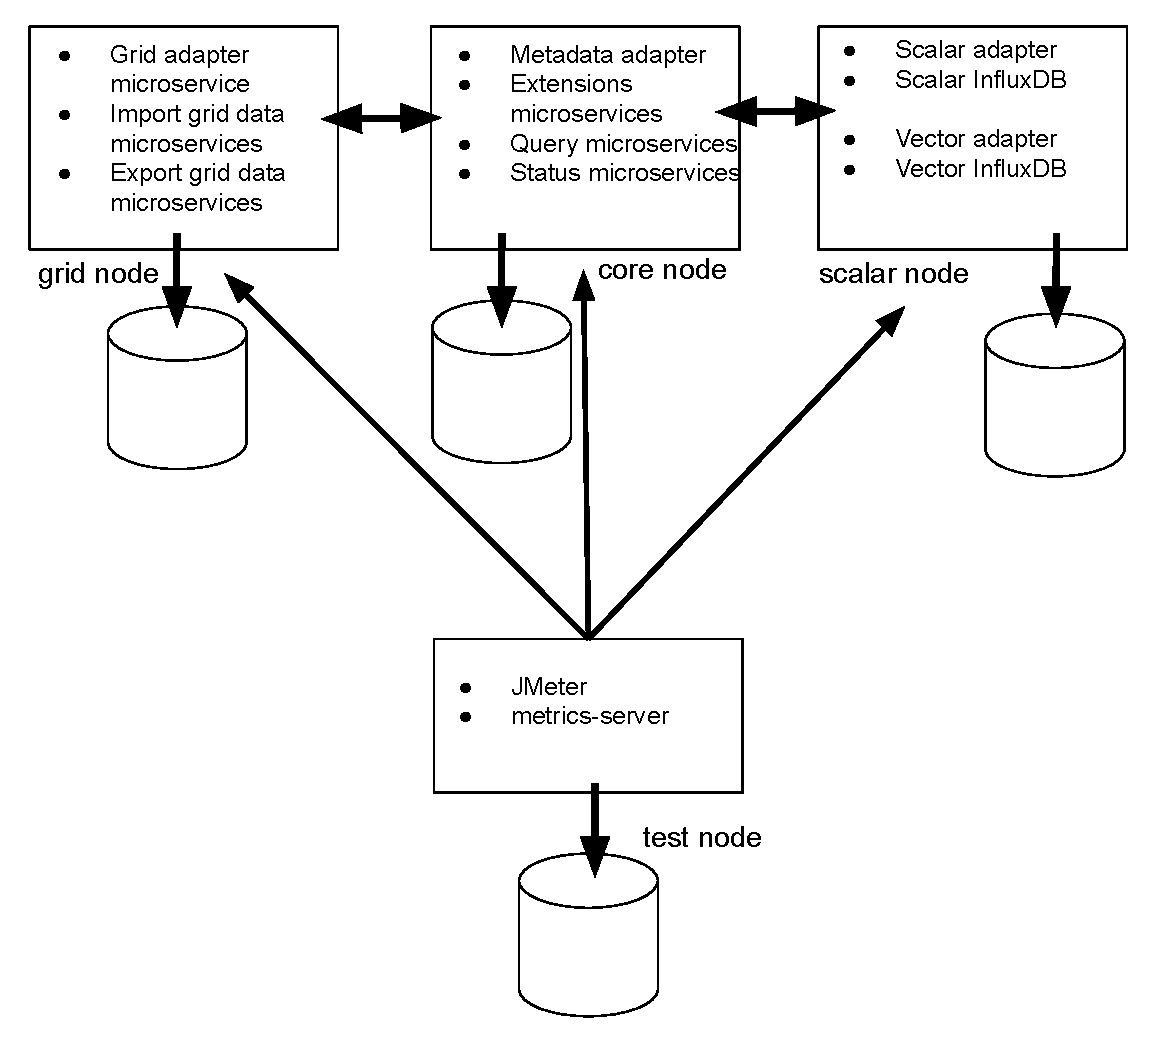
\includegraphics[width=0.75\textwidth]{results/work_load/eks_node_setup.pdf}
    \caption{\acrfull{eks} node setup}
    \label{fi:eks_node_setup}
\end{figure}

Users can use one of the above methods to schedule microservice on physical nodes for better performance. For the moment, we used node affinity to schedule the microservices. We chose the above method since it allows us to schedule all the microservices in a node when there is only a single physical node available. Microservices are assigned to each node in \cref{tab:aws_eks_nodes} based on the node label as below;
\begin{itemize}
    \item \emph{core} -- metadata, extensions, query, status and extension services
    \item \emph{grid} -- grid adapter, import and export grid data
    \item \emph{scalar} -- scalar and vector adapters, import and export of same data types
    \item \emph{test} --  JMeter and metric server
\end{itemize}
\cref{fi:eks_node_setup} shows the overview of the microservices assignment to each node in the \acrshort{eks} setup. Further, it shows the connectivity of the nodes and the data interactions via the arrows. We scheduled the microservices in the core labeled node together, since most of those services are communicating together, and running them inside one physical node reduces the latency. Then we separate scalar and vector microservices and their databases to separate the load from the core node while storing scalar and vector timeseries data. Similarly, we assigned microservices to grid and test nodes based on the higher bandwidth requirements.
